\documentclass[12pt]{article}
\usepackage{float}
\usepackage{caption, subcaption}
\usepackage[T1]{fontenc}
\usepackage[backend=bibtex, maxbibnames=99, sorting=none]{biblatex}
\addbibresource{sample.bib}
\usepackage{url}
\usepackage[utf8]{inputenc}
\usepackage{amsmath}
\usepackage{setspace}
\usepackage{graphicx}
\graphicspath{{Images/}}
\usepackage{parskip}
\usepackage{geometry}
\usepackage{array}
\usepackage{booktabs}
\usepackage{multirow}
\usepackage{enumitem}
\usepackage{amssymb}
\usepackage{framed}
\usepackage{fancyhdr}
\usepackage[colorlinks=true, linkcolor=blue, urlcolor=blue]{hyperref}
\usepackage{vmargin}
\usepackage{subcaption} %usamos subcaption mejor que subfig (más moderno)
\usepackage{eurosym}
\usepackage[table,xcdraw]{xcolor} % add color to your tables
\usepackage[bottom]{footmisc} %footnotes
\definecolor{blau}{RGB}{210,235,255}
\definecolor{blau2}{RGB}{120,170,225}
\setmarginsrb{2.5 cm}{2 cm}{2 cm}{2.5 cm}{1 cm}{0.5 cm}{1 cm}{1 cm}

\usepackage{multirow}

\usepackage{chngcntr}

\usepackage[framed, numbered]{matlab-prettifier}
 
\counterwithin{figure}{section}
\counterwithin{table}{section}
\numberwithin{equation}{section}

\usepackage{titlesec}
\usepackage{hyperref}
\usepackage{listings}
\usepackage{multicol}
\setlength{\columnsep}{1cm}

\titleclass{\subsubsubsection}{straight}[\subsection]

\newcounter{subsubsubsection}[subsubsection]
\renewcommand\thesubsubsubsection{\thesubsubsection.\arabic{subsubsubsection}}
\renewcommand\theparagraph{\thesubsubsubsection.\arabic{paragraph}} % optional; useful if paragraphs are to be numbered

\titleformat{\subsubsubsection}
  {\normalfont\normalsize\bfseries}{\thesubsubsubsection}{1em}{}
\titlespacing*{\subsubsubsection}
{0pt}{3.25ex plus 1ex minus .2ex}{1.5ex plus .2ex}

\makeatletter
\renewcommand\paragraph{\@startsection{paragraph}{5}{\z@}%
  {3.25ex \@plus1ex \@minus.2ex}%
  {-1em}%
  {\normalfont\normalsize\bfseries}}
\renewcommand\subparagraph{\@startsection{subparagraph}{6}{\parindent}%
  {3.25ex \@plus1ex \@minus .2ex}%
  {-1em}%
  {\normalfont\normalsize\bfseries}}
\def\toclevel@subsubsubsection{4}
\def\toclevel@paragraph{5}
\def\toclevel@paragraph{6}
\def\l@subsubsubsection{\@dottedtocline{4}{7em}{4em}}
\def\l@paragraph{\@dottedtocline{5}{10em}{5em}}
\def\l@subparagraph{\@dottedtocline{6}{14em}{6em}}
\makeatother

\usepackage[table,xcdraw]{xcolor}

\setcounter{secnumdepth}{4}
\setcounter{tocdepth}{4}


\usepackage{pdflscape} %Per poder posar la pàgina en horizontal
\usepackage{multicol} %Escriure en columnes 
 
	% Author
\date{\today}							% Date

\makeatletter
\let\thetitle\@title
\let\theauthor\@author
\let\thedate\@date
\makeatother

\pagestyle{fancy}
\fancyhf{}
\lhead{22DM014 - Intro to Natural Language Processing}
\rhead{Analysis of Amazon Books and Review}
\cfoot{\thepage}

\begin{document}

\begin{titlepage}
	\centering
    
\includegraphics[scale = 0.7]{bse_logo.png}\\[1.2 cm]	% University Logo
    \textsc{\LARGE Barcelona School of Economics}\\[2.0 cm]	% University Name
	\textsc{\Large Data Science Methodology Program}\\[0.5 cm]				% Course Code
	\textsc{\large 22DM014 - Intro to Natural Language Processing }\\[0.5 cm]				% Course Name
	\rule{\linewidth}{0.2 mm} \\[0.4 cm]
	{ \huge \bfseries Analysis of Amazon Books and Reviews }\\
	\rule{ \linewidth}{0.2 mm} \\[1.5 cm]
	
\begin{center}
    
{ \emph{Authors: }\\
    \textsc{Chen}, Joshua \\
    \textsc{El Daou}, Mahmoud \\ 
    \textsc{Gallegos}, Rafael \\} 

\vspace{0.7cm}
    \textit{Professors:}\\  \textsc{Mueller}, Hannes \\
    	\textsc{Garcia}, Luis
        \\ \vspace{0.5cm}
\vspace{1.7cm}

 \end{center}
	\vfill
	
\end{titlepage}
	
\tableofcontents
\vspace{1cm}
\listoffigures
\listoftables
\pagebreak

\newpage

\section{Introduction}

On July 16th, 1995, Amazon opened as an online book retailer, promoting itself as "the world's biggest bookstore". Since then, Amazon has clearly expanded into other ventures but still remains the largest seller of books in the world. Amazon generates \$28 billion worldwide every year with a selection of over 32 million books. With Kindle and Audible, Amazon also has majority control of the ebook and audiobook markets as well. While Amazon is no longer primarily known as predominantly a bookseller, they have succeeded in becoming the most dominant bookstore in the world.

In 2013, Amazon acquired Goodreads, a social cataloging platform for books. Goodreads now has more than 150 million users and has become a cornerstone (for better or worse) in the book community. However, the partnership between world's largest bookseller and the largest community of readers, gives us the opportunity to acquire and use lots of book data to identify book trends and reader preferences.

\section{Literature Reviews}

\section{Dataset}

In this project, we explore the Amazon Books Reviews dataset, which can be found on Kaggle at the following link: \href{https://www.kaggle.com/datasets/mohamedbakhet/amazon-books-reviews}{Amazon Books Reviews Dataset}

Contained here are two large data sets contain information about Books and information about Reviews.


\begin{figure}[htbp]
    \centering
    \begin{minipage}{.45\linewidth}
        \subcaptionbox{Book Dataset}{
            \begin{tabular}{>{\raggedright}p{2.5cm}p{5cm}}
                \toprule
                \textbf{Feature} & \textbf{Description} \\
                \midrule
                Title & Book Title \\
                Descripe & Description of the book \\
                authors & Name of book authors \\
                image & URL for book cover \\
                previewLink & Link to access this book on Google Books \\
                publisher & Name of the publisher \\
                publishedDate & The date of publish \\
                infoLink & Link to get more information about the book on Google Books \\
                categories & Genres of books \\
                ratingsCount & Averaging rating for the book \\
                \bottomrule
            \end{tabular}
        }
    \end{minipage}\hfill
    \begin{minipage}{.45\linewidth}
        \subcaptionbox{Review Dataset}{
            \begin{tabular}{>{\raggedright}p{2cm}p{5cm}}
                \toprule
                \textbf{Feature} & \textbf{Description} \\
                \midrule
                id & The Id of the Book \\
                Title & Book Title \\
                Price & The Price of the Book \\
                User\_id & Id of the user who rates the book \\
                profileName & Name of user who rates the book \\
                helpfulness & Helpfulness rating of the review, e.g., 2/3 \\
                score & Rating from 0 to 5 for the book \\
                time & Time of giving the review \\
                summary & The summary of a text review \\
                text & The full text of a review \\
                \bottomrule
            \end{tabular}
        }
    \end{minipage}
\end{figure}

There are 214,404 books in the book dataset and 3,000,000 reviews in the review dataset. Clearly, two very large datasets, we subsetted the datasets and reviews to only the most relevant for our purposes.

First we dropped all the books without any ratings or descriptions as these are irrelevant for our purpose. This reduced the amount of books to 45,127. We then dropped any books with less than 10 reviews, considering them insignificant enough. Furthermore, using the \textit{Langid} package in Python, we removed any books that were identified to be any language other than English. This leaves us with 6,399 books.

We only kept the reviews that were for one of our 6,399 books and used the same method to remove non-English reviews. Because Goodreads allows other users to review other people's reviews, we used this to further subset only the most relevant reviews. Any reviews with less than 10 responses were therefore removed. This brought our review count to 94,573.

\section{Exploratory Data Analysis}

\begin{figure}
    \begin{minipage}[b]{0.5\linewidth}
    \centering
    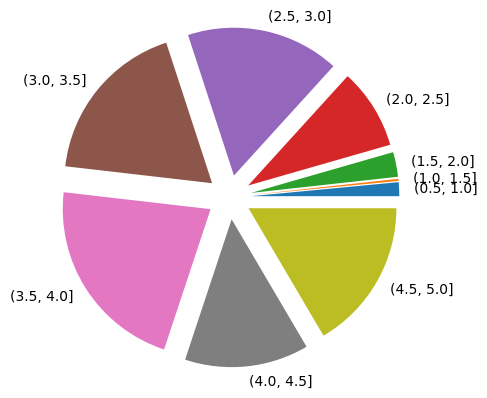
\includegraphics[width=0.99\textwidth]{percent_book_reviews.png}
    \caption{Percent of Books by Average Score}
\end{minipage}
    \hspace{0.01cm}
\begin{minipage}[b]{0.45\linewidth}
    \centering
    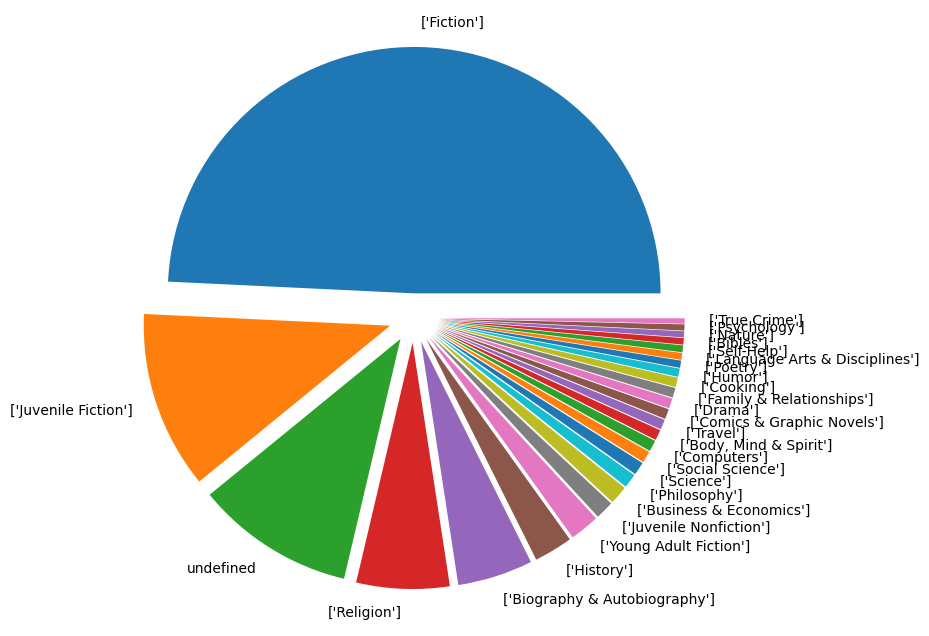
\includegraphics[width=1.2\textwidth]{genre_counts.png}
    \caption{Percentage of Books by Genre}
    \end{minipage}

\end{figure}
   \begin{figure}[ht]
    \begin{minipage}[b]{0.49\linewidth}
    \centering
    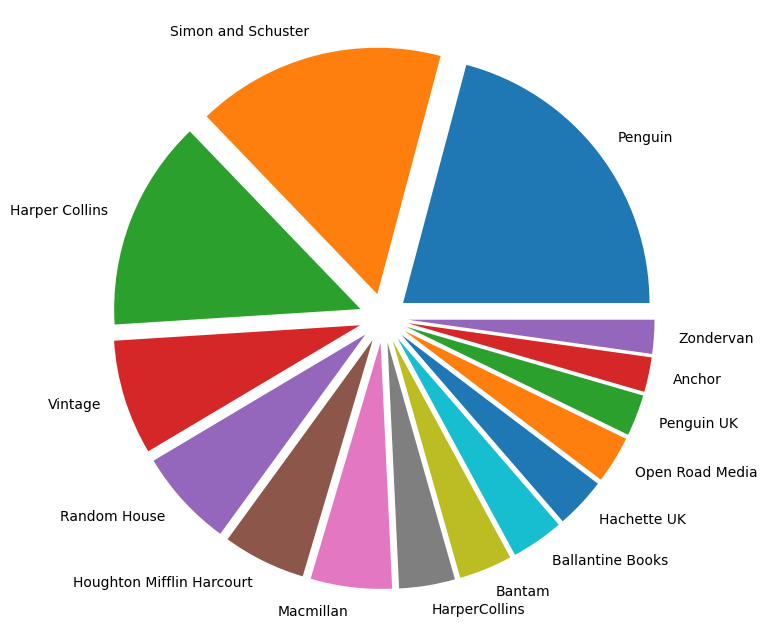
\includegraphics[width=0.99\textwidth]{publisher_counts.png}
    \caption{Percentage of Books by Publisher}
   \end{minipage}
    \hspace{0.01cm}
\begin{minipage}[b]{0.49\linewidth}
    \centering
    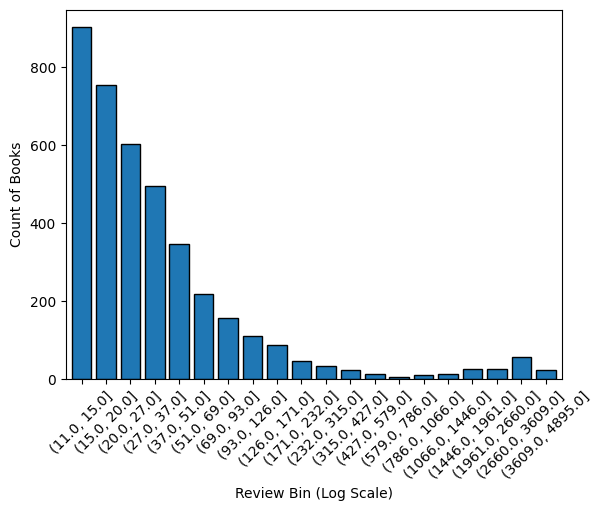
\includegraphics[width=0.99\textwidth]{reviewcount.png}
    \caption{Percentage of Books by Publisher}
    \end{minipage}
\end{figure}

First, to better understand the dataset we performed some exploratory data analysis. By calculating the average review scores for each book, we find that the largest representation of reviews are within the 3.0 - 4.0 range, with a significant majority of the books receiving a rating above 3.0. The median rating was a 3.6 and the mean was also around 3.6. While this in balance may be reflective of our selection bias of only the most reviewed books (i.e. the most popular books), it is typical for people to tend towards higher reviews as people selectively consume things they tend to enjoy rather than sampling randomly (ex. MovieLens dataset).

By genre we see that the majority of the books are fiction. However, this is only broken down into Juvenile Fiction, Young Adult Fiction, and Fiction whereas non-fiction books are broken down into many topics/subtopics. Genres with less than 15 books were grouped into "Other" as there were a number of hyper-specfiic or uninformative genres. Particularly amusing ones include "Fairy", "Diners", "Bachelors", and "Human-computer Interaction".

We also have the breakdown by publishers. While this was not utilized in this paper, an interesting extension of this project would be to use the description data to see if there are any significant differences among how different publishers market their books. 

Finally, we have the counts of books by the number of reviews they received (binned by a log 10 scale). Here we see that a significant majority of the books have received less than 100 reviews. However, there is a significant tail with the maximum review count reaching 4,895.


\begin{figure}
    \centering
    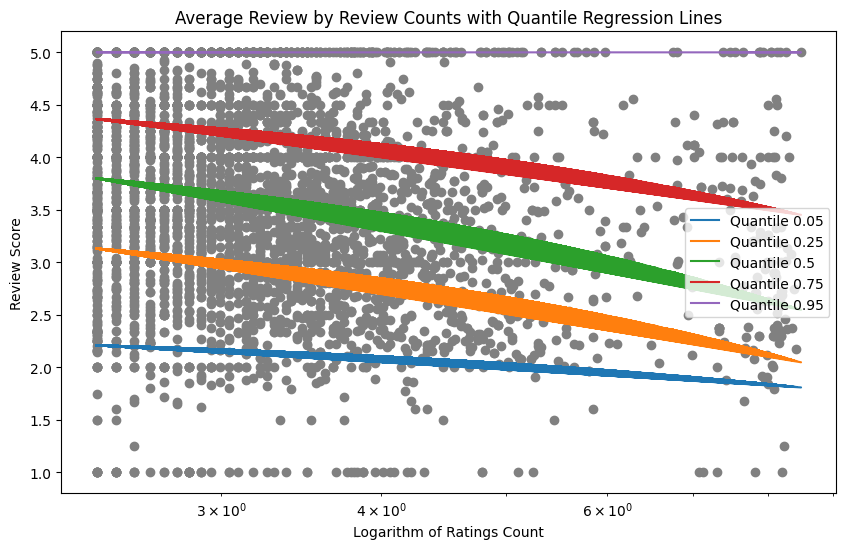
\includegraphics[scale=0.58]{quantreg_reviewscore.png}
\caption{Quantile Regression of Average Reviews per Book over Count of Reviews} 
\end{figure}

\subsection{Descriptions}

\subsubsection{New York Times Bestsellers}

\subsection{Reviews}
In the reviews, there are two important text features - the review summary and the full review itself.


\subsubsection{Sentiment Analysis}

\begin{figure}
    \centering
    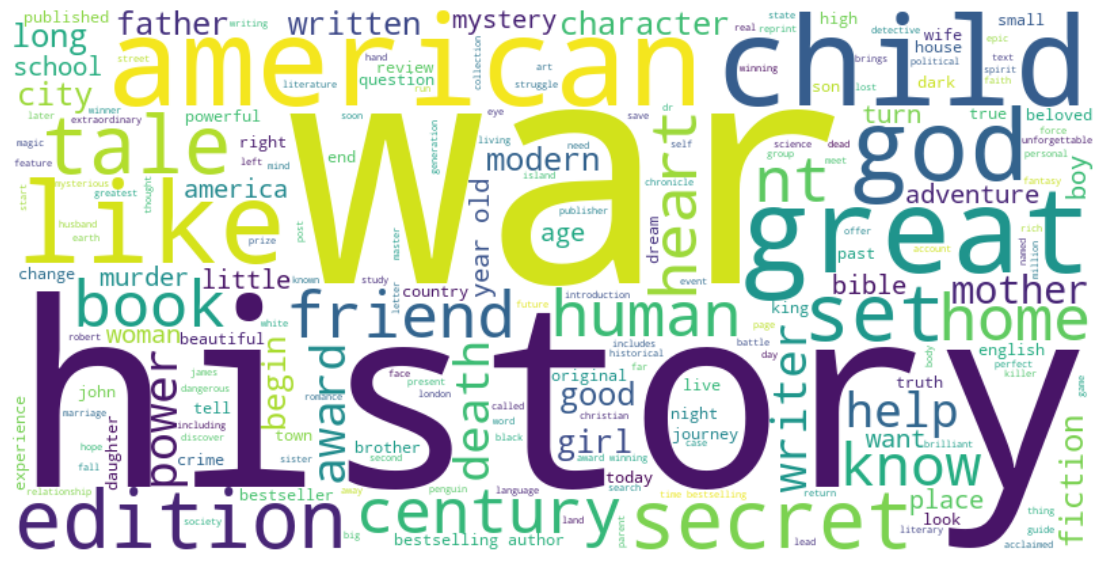
\includegraphics[scale=0.58]{bow_descriptions.png}
    \caption{Bag of Words - Book Descriptions - MinDF = 20, MaxDF = 0.01}
\end{figure}

\section{Predicting Review Score from Text}

\section{Review Description Alignment}

\section{Conclusions}
\vspace{1em} 


%\bibliographystyle{plain}
%\bibliography{Bibliography.bib}

\newpage
\printbibliography[heading=bibintoc]

\end{document}